\chapter{Measuring \texorpdfstring{\ARaw}{ARaw}}
\label{chap:cpv:araw}

In order to calculate \dACP, \ARaw must first be measured for each mode.
This is the asymmetry in the positively- and negatively-charged \PLambdac\ 
yields, as in \cref{eqn:cpv:theory:araw}.
The yields are measured with \chisq\ fits to the \PLambdac\ and \APLambdac\ 
mass spectra, in a similar manner to the fit to the charge-combined sample 
discussed in \cref{chap:cpv:prelim_fits}.
The weights from the kinematic weighting, from 
\cref{chap:cpv:kinematic_weighting}, and the phase space efficiency correction, 
from \cref{chap:cpv:phsp}, are used in the fits such that the bin contents 
$b_{i}$, to which to fit model is compared, is
\begin{equation}
  b_{i} = \sum_{j = 1}^{N_{i}} \frac{%
    w_{j}(\pT^{\PLambdac}, \Eta^{\PLambdac},
          \pT^{\Pproton}, \Eta^{\Pproton})
  }{%
    \eff_{j}(\msqphm, \msqhh, \thetap, \phip, \phihh)
  },
\end{equation}
where $N_{i}$ is the number of candidate decays in the $i$th \phh\ mass bin, 
$w_{j}$ is per-candidate kinematic weight for the $j$th candidate in the $i$th 
bin, and $\eff_{j}$ is the efficiency.

To try to reduce the effects of experimenter bias, the fitted central values of 
\ARaw\ are \emph{blinded}, and cannot be inspected until they are 
\emph{unblinded}.
To be able to assess the quality of the fit results without inadvertently 
unblinding the result, only the fit to \PLambdac\ data is inspected.
For the \APLambdac data, only the pull distribution of the fit with respect to 
the data is inspected, as this is not biasing but still indicates the fit 
quality.
The specific method used to blind the central value is discussed in 
\cref{chap:cpv:araw:blinding}.

\section{Simultaneous fit}
\label{chap:cpv:araw:simultaneous_fit}

Simultaneously fits are performed on the charge-separated \PLambdac\ and 
\APLambdac\ samples, measuring \ARaw\ by including it as a parameter in the 
fit.
This is advantageous as it increases the statistical sensitivity of the 
measurement, as all the data is considered at once, and the error analysis is 
taken care of by the fitter.
The alternative approach is to perform two separate fits and calculate \ARaw\ 
explicitly using the two measured yields.
This introduces the complexity of having to blind at least two quantities (one 
of the yields and \ARaw), as opposed to blinding the single \ARaw\ parameter in 
a simultaneous fit.

The fit model for each charge is created as a clone of a `master' \ac{PDF}, 
whose signal and background components are identical to those described in 
\cref{chap:cpv:prelim_fits}.
Before creating the two models, one per charge, it is specified which 
parameters of the master \ac{PDF} are to become charge-specific.
As the \PLambdac\ final states are not \CP\ conjugates of themselves, the 
matter final state may interact differently with the detector than the 
antimatter final state, and hence they may have different mass resolutions.
This motivates the splitting of all of the signal model parameters $\alpha$, 
$\mu$, $\sigma_{1}$, and $\sigma_{2}$.
Likewise, the background composition can be different for the positively- and 
negatively-charged final states, and so the background model parameter $a_{0}$ 
is also split.
The signal \ac{PDF}, $f_{+}$ for \PLambdac\ and $f_{-}$ for \APLambdac, is then
\begin{equation}
  f_{\pm}(x; \mu_{\pm}, w_{\pm}, \alpha_{\pm}) =
    \alpha_{\pm}{}G(x; \mu_{\pm}, \alpha_{\pm}w_{\pm}) +
    (1 - \alpha_{\pm})G(x; \mu_{\pm}, \frac{\alpha_{\pm}}{w_{\pm}}),
\end{equation}
and the corresponding background \ac{PDF} is
\begin{equation}
  g_{\pm}(x) = a_{\pm,0}x,
\end{equation}
as in \cref{eqn:cpv:prelim_fits:sig_model} 
and~\cref{eqn:cpv:prelim_fits:bkg_model}.
The width parameters $\sigma_{\pm, 1}$ and  $\sigma_{\pm, 2}$ of the signal 
model are defined as in \cref{eqn:cpv:prelim_fits:sigma_def}.

The total \ac{PDF} for each charge is
% TODO should use \nsig and \nbkg
\begin{equation}
  h_{\pm}(x) = \nsigpm f_{\pm}(x) + \nbkgpm g_{\pm}(x),
\end{equation}
where the signal and background yields are parameterised as
\begin{align}
  \nsigpm &= \frac{1}{2}\nsig(1 \pm \ARaw),\\
  \nbkgpm &= \frac{1}{2}\nbkg(1 \pm \ARawBg).
\end{align}
Here, \nsig\ and \nbkg\ are the signal and background yields for the 
\emph{combined} \PLambdac\ and \APLambdac\ sample.
This parameterisation of the charge-specific yields permits $\ARaw$ to measured 
directly from in fit.

The fully selected data are used, with one simultaneous fit performed for each 
year and magnet polarity sub-sample.
The data are weighted by the kinematic weights as described in 
\cref{chap:cpv:kinematic_weighting}.
The loss function is defined as a \chisq, which is minimised with \minuit\ and 
a covariance matrix is computed with \hesse.
A \chisq\ fit is chosen over a binned maximum likelihood fit as a \chisq\ fit 
handles weights more naturally, in particular the evaluation of the covariance 
matrix is considerably simpler, as discussed in 
\cref{chap:cpv:prelim_fits:least_squares}.

\section{Blinding}
\label{chap:cpv:araw:blinding}

With \ARaw\ a parameter of the simultaneous fit, its value should be hidden 
from the fit results in order not to bias the experimenter.
This is done by fitting a variable as the \emph{transform} of \ARaw.
The transformation itself can be adding some random offset to the central 
value, or changing its order of magnitude, but it is applied in such a way as 
to leave the uncertainty on the parameter estimate unchanged.
Only the transformed value that is reported, leaving the unblinded value 
hidden.

This analysis applies a linear blinding offset, transforming the unblinded 
central value $x$ as
\begin{equation}
  x' = x + \beta\xi,
\end{equation}
where $\xi$ is a number sampled from a normal distribution with mean zero and 
unit width, and $\beta$ is a known scaling parameter, which is chosen to be 
$0.25$.
The number $\xi$ is chosen deterministically from a string in the fitting 
program, such that the same input string always gives the same $\xi$, but in a 
way that the smallest changes in the input change the output unpredictably.
In this way, the string is effectively the seed for a random number generator, 
and $\xi$ is the first number returned by the generator.
Different strings are used for different modes, but are the same for the fits 
to the different data sub-samples.
% The string used for the \pKK mode is \texttt{2ONNiFZLqk4yvv6ovBeg} and the 
% string used for the \ppipi mode is \texttt{4VjezpHK0wzlZ6qbeolq}.

As the blinding offsets are different for each mode, the difference between 
$\ARaw(\pKK)$ and $\ARaw(\ppipi)$, that is \dACP, is also blinded.
However, the difference between two blinded values of \dACP\ is equal to the 
difference between the unblinded values.
This is useful for systematic studies, which will be described in 
\cref{chap:cpv:syst}.
Similarly, as the blinding parameters are the same for all data sub-samples, it 
is still meaningful to compare blinded values of \ARaw and \dACP between them 
to check for consistency, as the differences are not blinded.

In addition to blinding the values of \ARaw\ and \dACP, the plots of the fits 
to the \APLambdac\ data are blind (as comparing \PLambdac\ and \APLambdac\ fits 
side-by-side would allow one to infer the size of the asymmetry), as are plots 
of the data and model asymmetry in bins of \PLambdac\ mass.
The pull plots and \chisq\ values are not blinded it the fit presentations as 
they do not indicate the asymmetry value.

\section{Fit results}
\label{chap:cpv:araw:results}

Fits to the \pKK\ and \ppipi\ 2012 magnet down data are shown in 
\cref{fig:cpv:araw:fits:pKK,fig:cpv:araw:fits:ppipi}.
The corresponding correlation matrices for the fits are given in 
\cref{fig:cpv:araw:correlation}.

\begin{figure}
  \begin{subfigure}[b]{0.5\textwidth}
    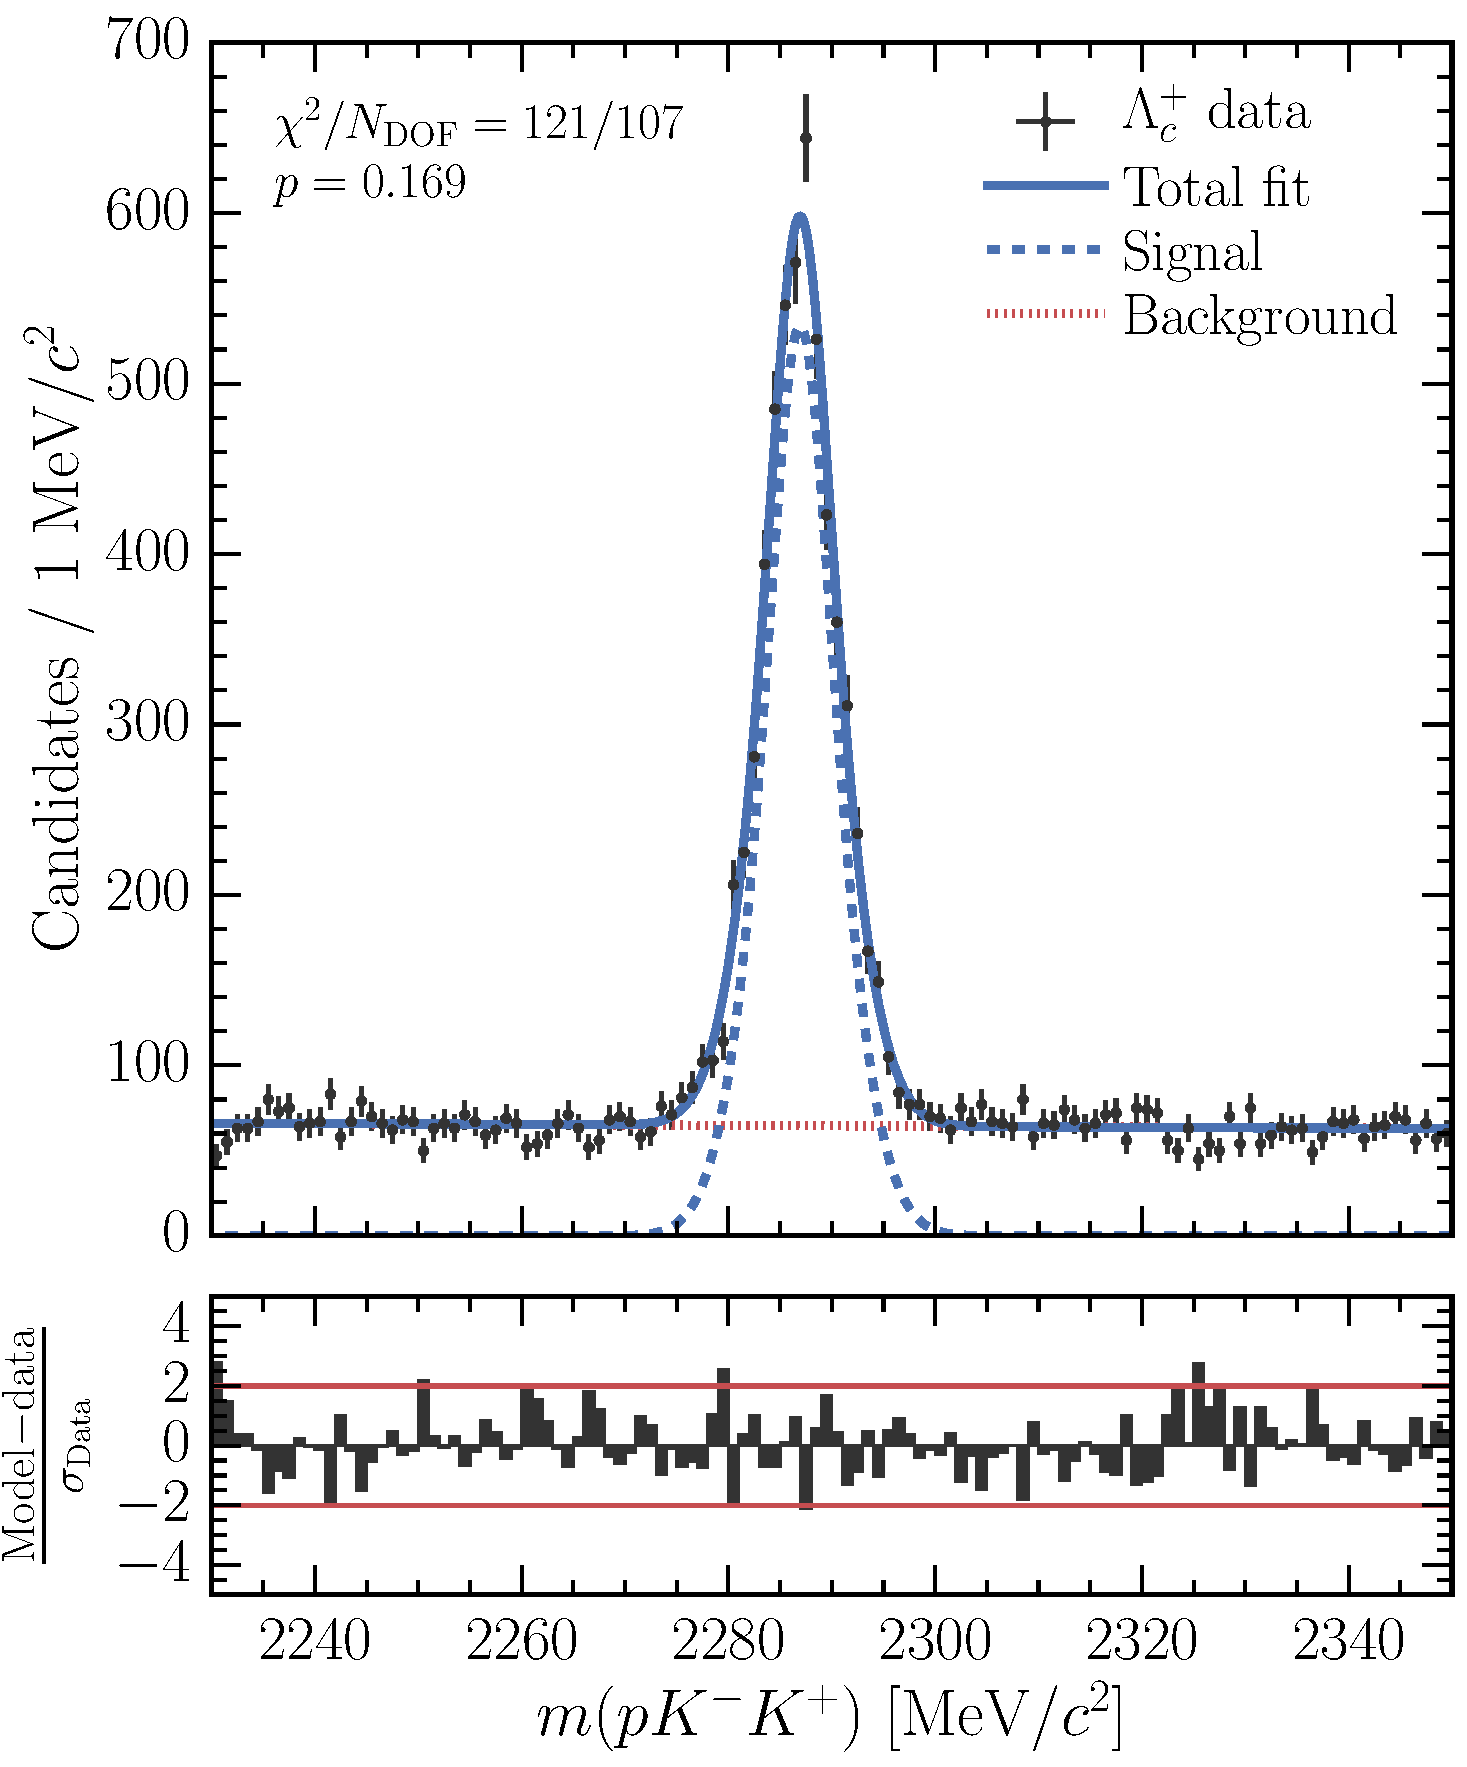
\includegraphics[width=\textwidth]{cpv/araw/LcTopKK_2012_MagDown_fit-Lcp.pdf}
    \caption{\PLambdac}
    \label{fig:cpv:araw:fits:pKK:Lcp}
  \end{subfigure}
  \begin{subfigure}[b]{0.5\textwidth}
    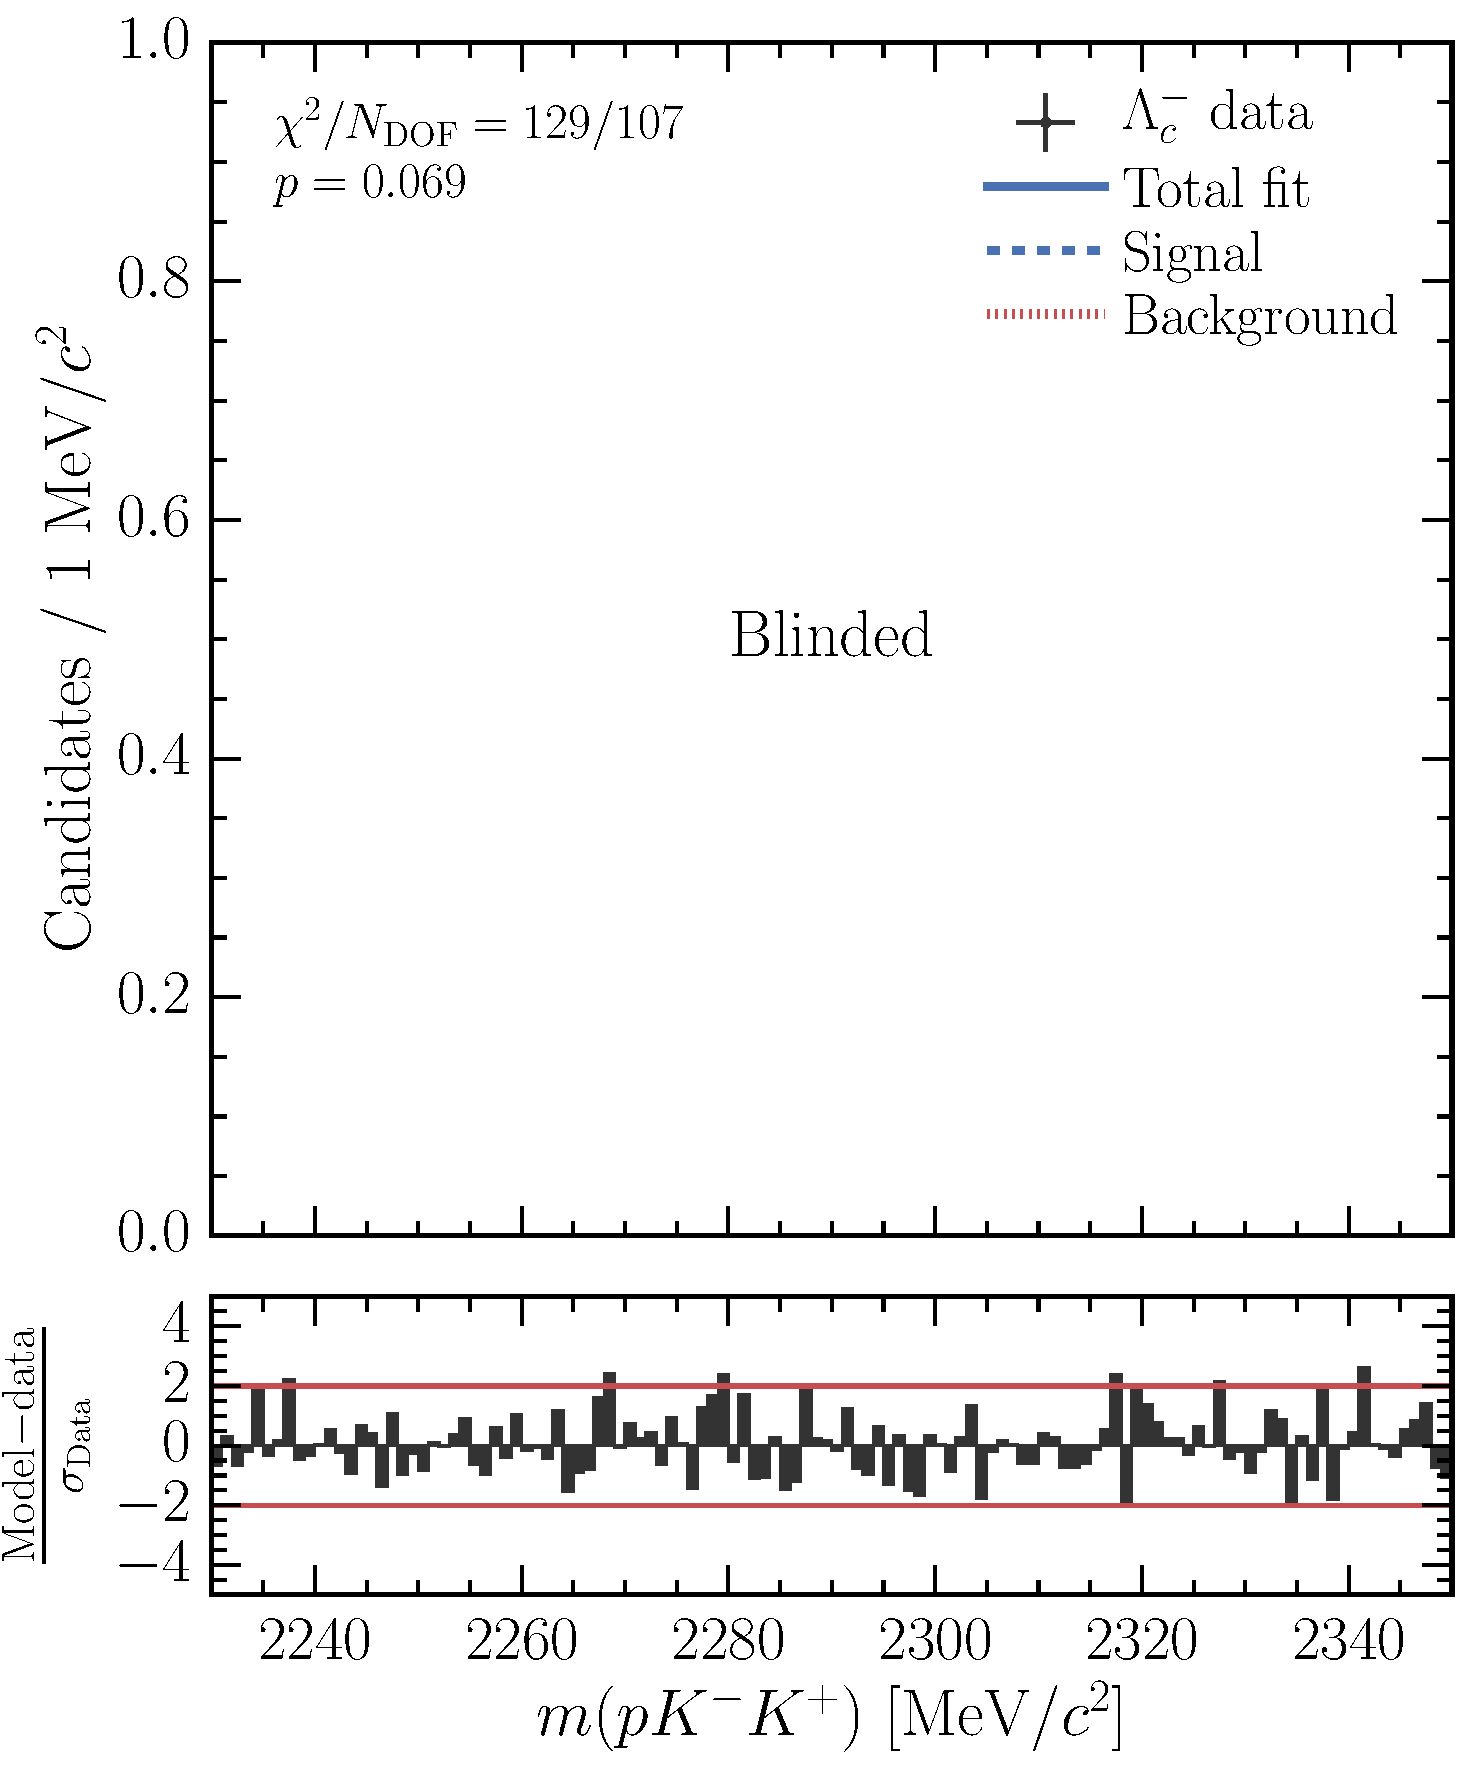
\includegraphics[width=\textwidth]{cpv/araw/LcTopKK_2012_MagDown_fit-Lcm.pdf}
    \caption{\APLambdac}
    \label{fig:cpv:araw:fits:pKK:Lcm}
  \end{subfigure}
  \begin{subfigure}[b]{0.5\textwidth}
    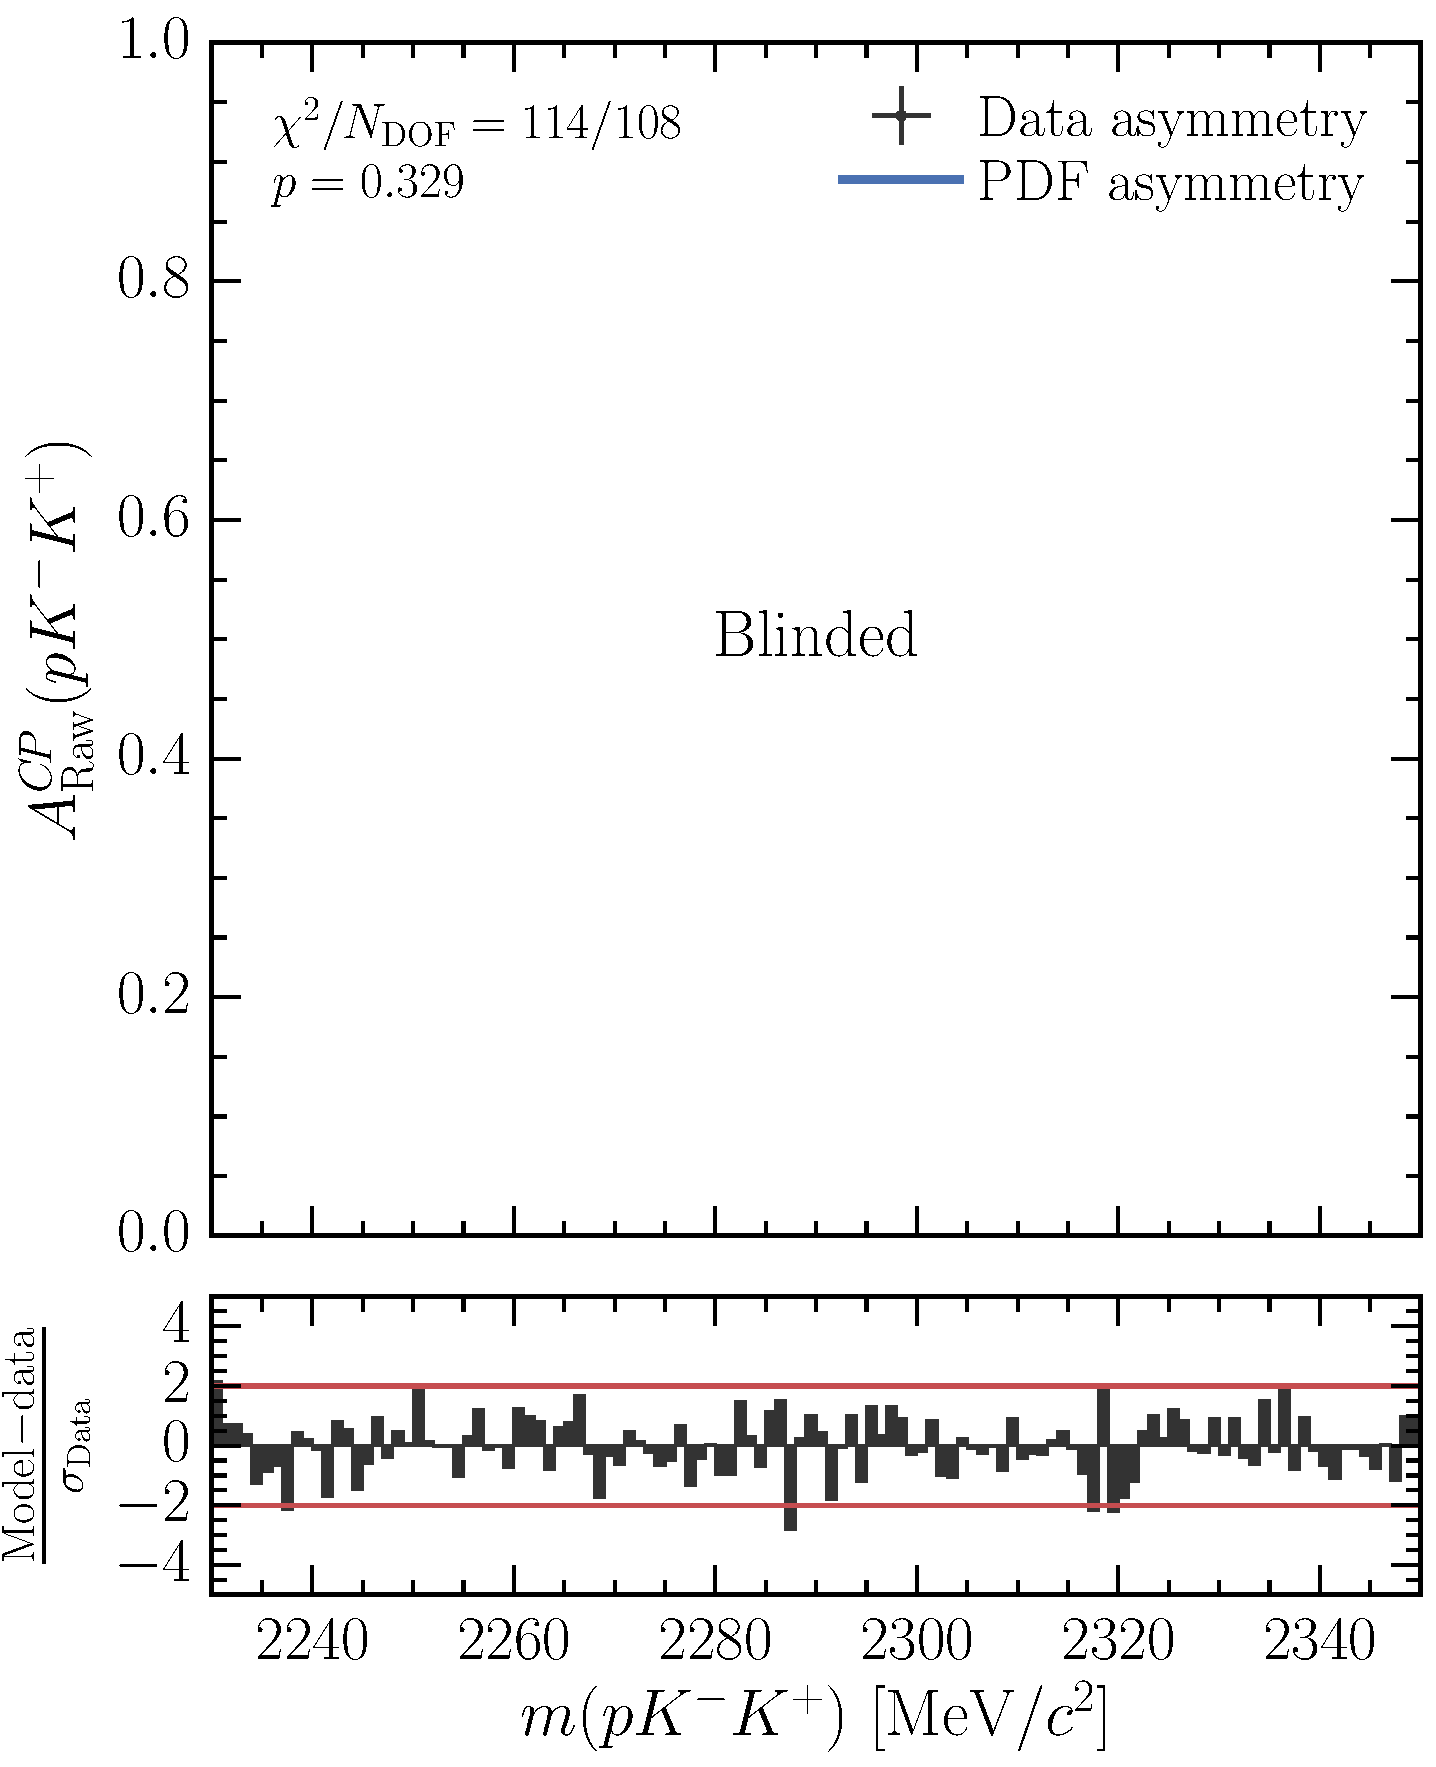
\includegraphics[width=\textwidth]{cpv/araw/LcTopKK_2012_MagDown_fit_pdf_araw.pdf}
    \caption{\ARaw}
    \label{fig:cpv:araw:fits:pKK:ARaw}
  \end{subfigure}
  \caption{%
    Results of the simultaneous fit to the \pKK\ 2012 magnet down dataset.
    The difference between the \PLambdac\ data and model 
    (\subref*{fig:cpv:araw:fits:pKK:Lcp}) and the \APLambdac\ data and model 
    (\subref*{fig:cpv:araw:fits:pKK:Lcm}) is shown in the bottom 
    plot~(\subref*{fig:cpv:araw:fits:pKK:ARaw}).
    The full offline selection is applied.
    The solid blue line is the total fit to the data in black points, and the 
    dotted red and dashed blue lines are the background and signal components, 
    respectively.
    Below each fit is a pull plot, showing the difference between the total fit 
    model and the data in each bin, normalised by the Poisson uncertainty on 
    the number of entries in that bin.
  }
  \label{fig:cpv:araw:fits:pKK}
\end{figure}

\begin{figure}
  \begin{subfigure}[b]{0.5\textwidth}
    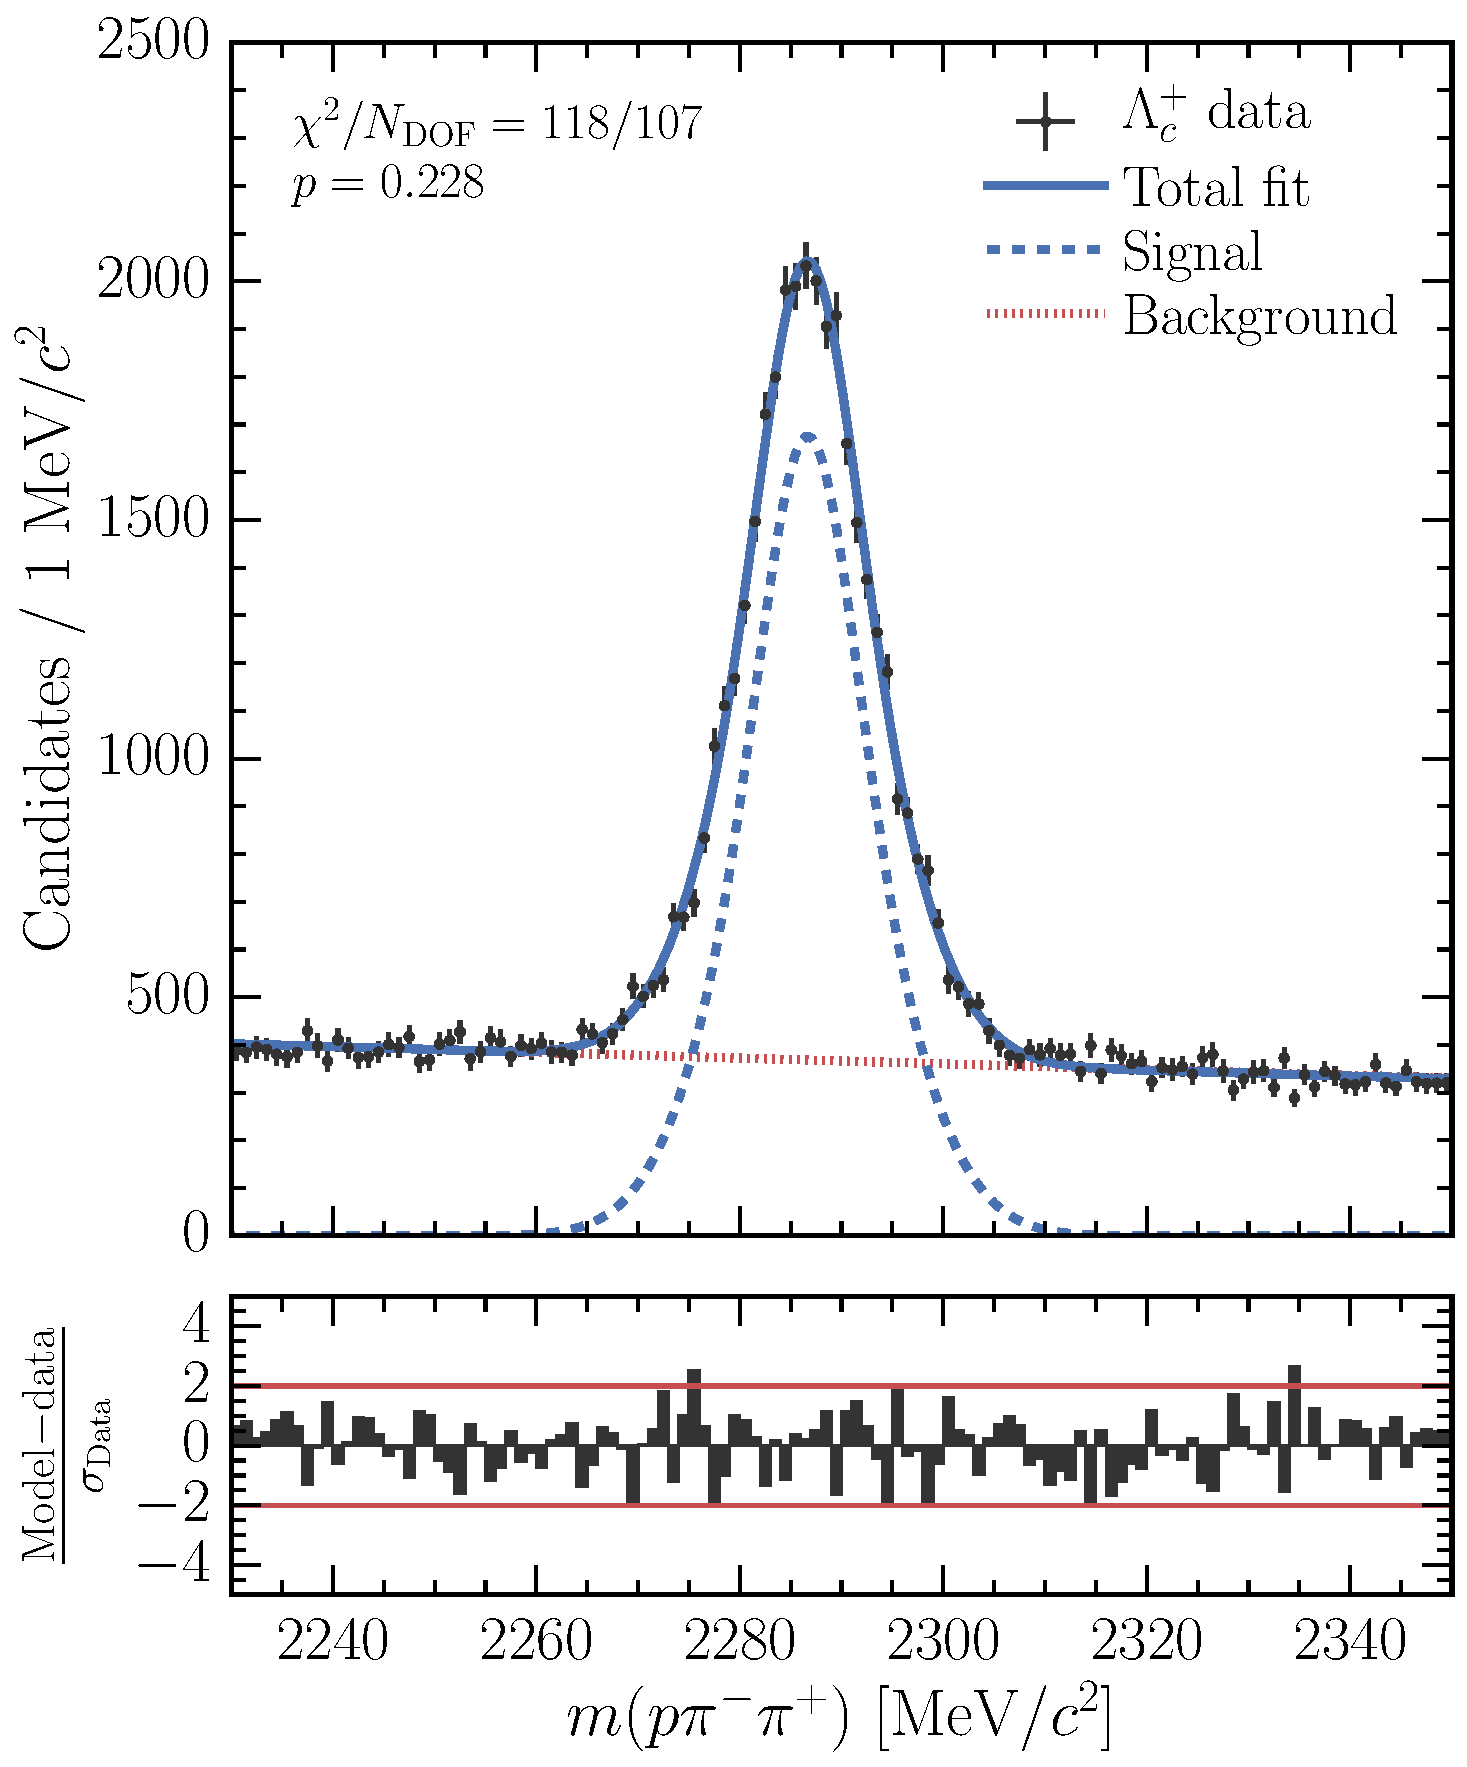
\includegraphics[width=\textwidth]{cpv/araw/LcToppipi_2012_MagDown_fit-Lcp.pdf}
    \caption{\PLambdac}
    \label{fig:cpv:araw:fits:ppipi:Lcp}
  \end{subfigure}
  \begin{subfigure}[b]{0.5\textwidth}
    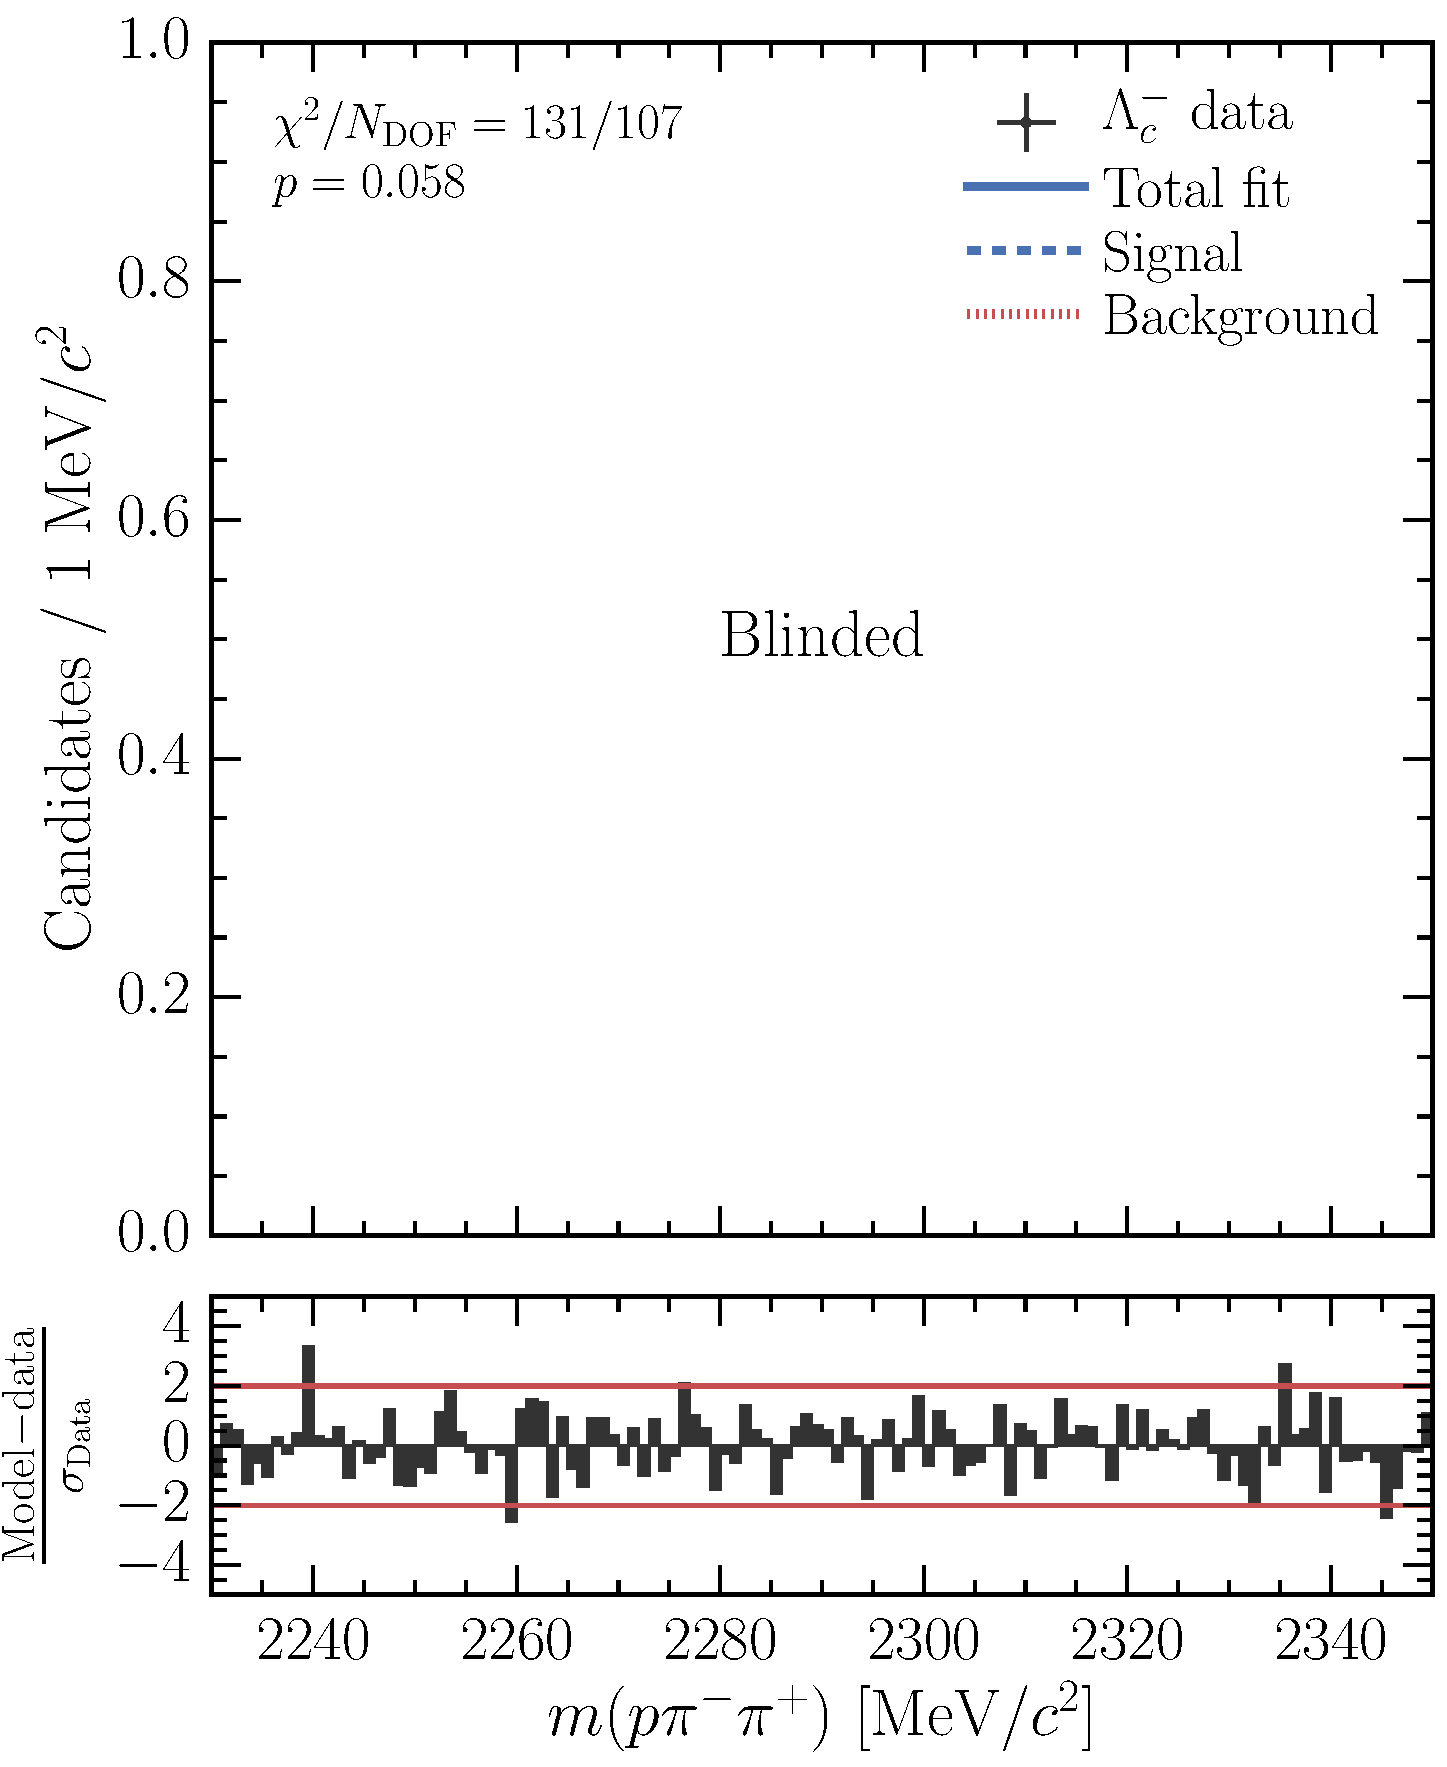
\includegraphics[width=\textwidth]{cpv/araw/LcToppipi_2012_MagDown_fit-Lcm.pdf}
    \caption{\APLambdac}
    \label{fig:cpv:araw:fits:ppipi:Lcm}
  \end{subfigure}
  \begin{subfigure}[b]{0.5\textwidth}
    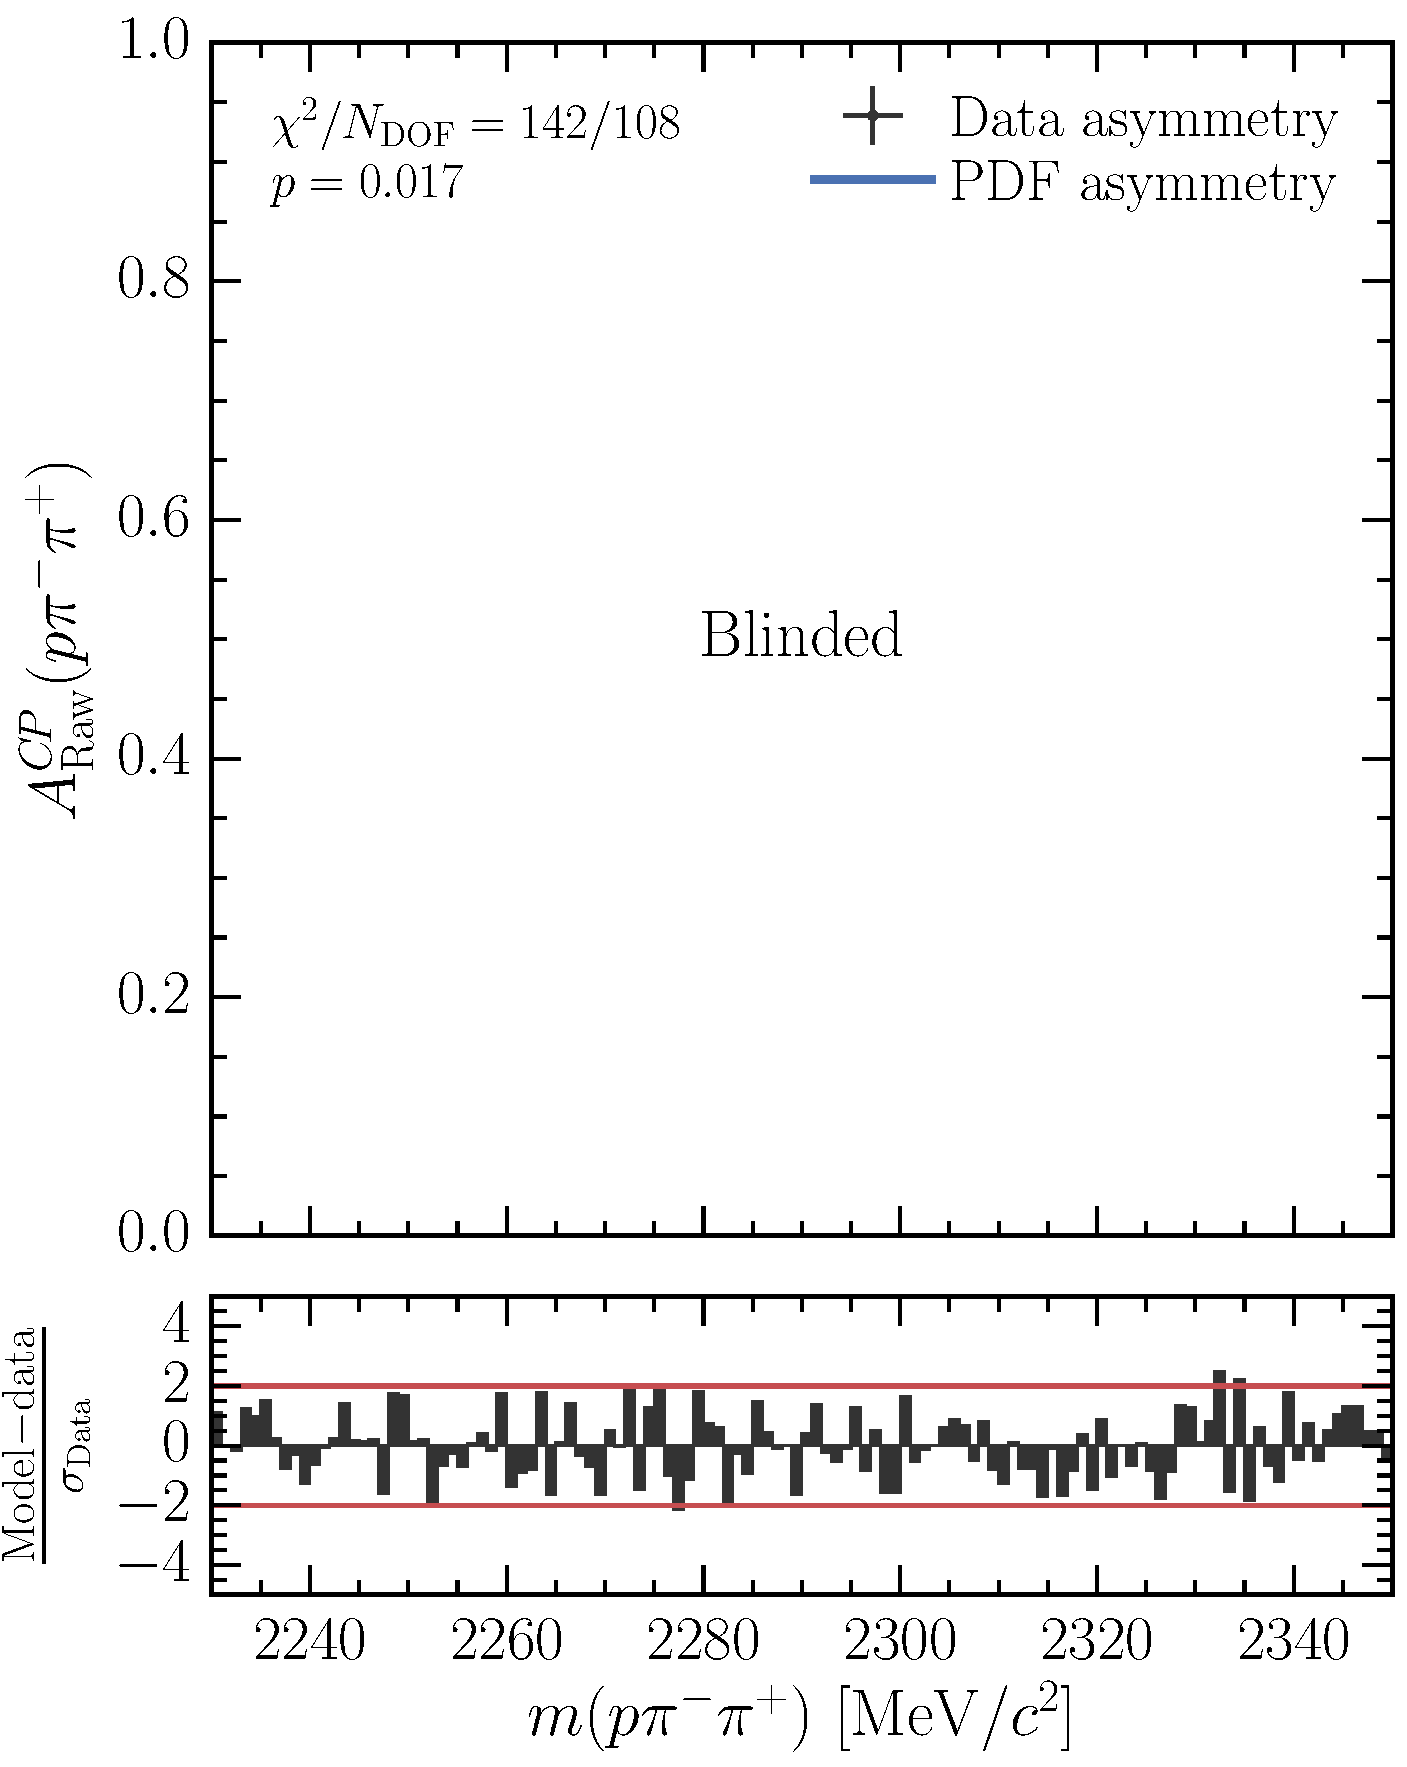
\includegraphics[width=\textwidth]{cpv/araw/LcToppipi_2012_MagDown_fit_pdf_araw.pdf}
    \caption{\ARaw}
    \label{fig:cpv:araw:fits:ppipi:ARaw}
  \end{subfigure}
  \caption{%
    Results of the simultaneous fit to the \ppipi\ 2012 magnet down dataset.
    The difference between the \PLambdac\ data and model 
    (\subref*{fig:cpv:araw:fits:ppipi:Lcp}) and the \APLambdac\ data and model 
    (\subref*{fig:cpv:araw:fits:ppipi:Lcm}) is shown in the bottom 
    plot~(\subref*{fig:cpv:araw:fits:ppipi:ARaw}).
    The full offline selection is applied.
    The solid blue line is the total fit to the data in black points, and the 
    dotted red and dashed blue lines are the background and signal components, 
    respectively.
    Below each fit is a pull plot, showing the difference between the total fit 
    model and the data in each bin, normalised by the Poisson uncertainty on 
    the number of entries in that bin.
  }
  \label{fig:cpv:araw:fits:ppipi}
\end{figure}

\begin{figure}
  \begin{center}
    \begin{subfigure}[b]{0.6\textwidth}
      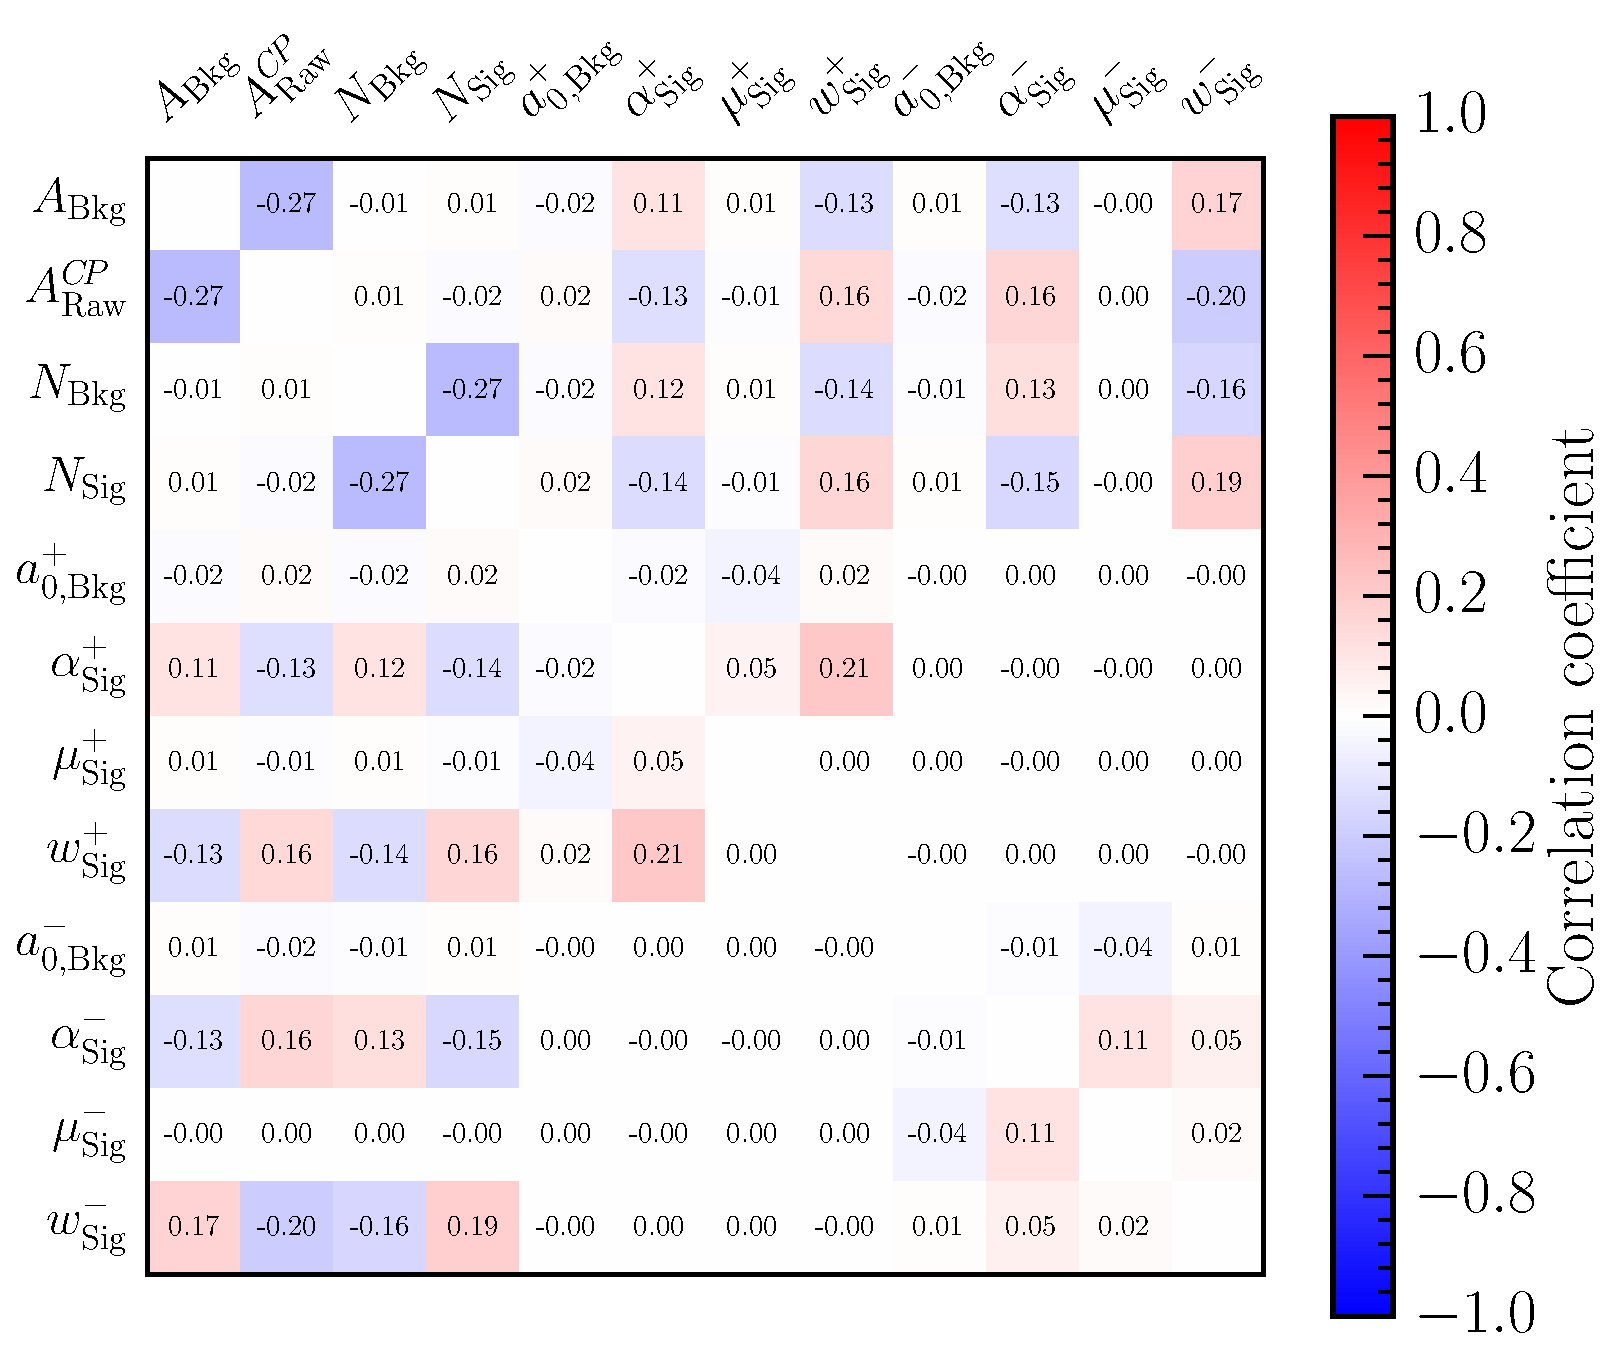
\includegraphics[width=\textwidth]{cpv/araw/LcTopKK_2012_MagDown_correlation_matrix.pdf}
      \caption{\pKK}
      \label{fig:cpv:araw:correlation:pKK}
    \end{subfigure}\\
    \begin{subfigure}[b]{0.6\textwidth}
      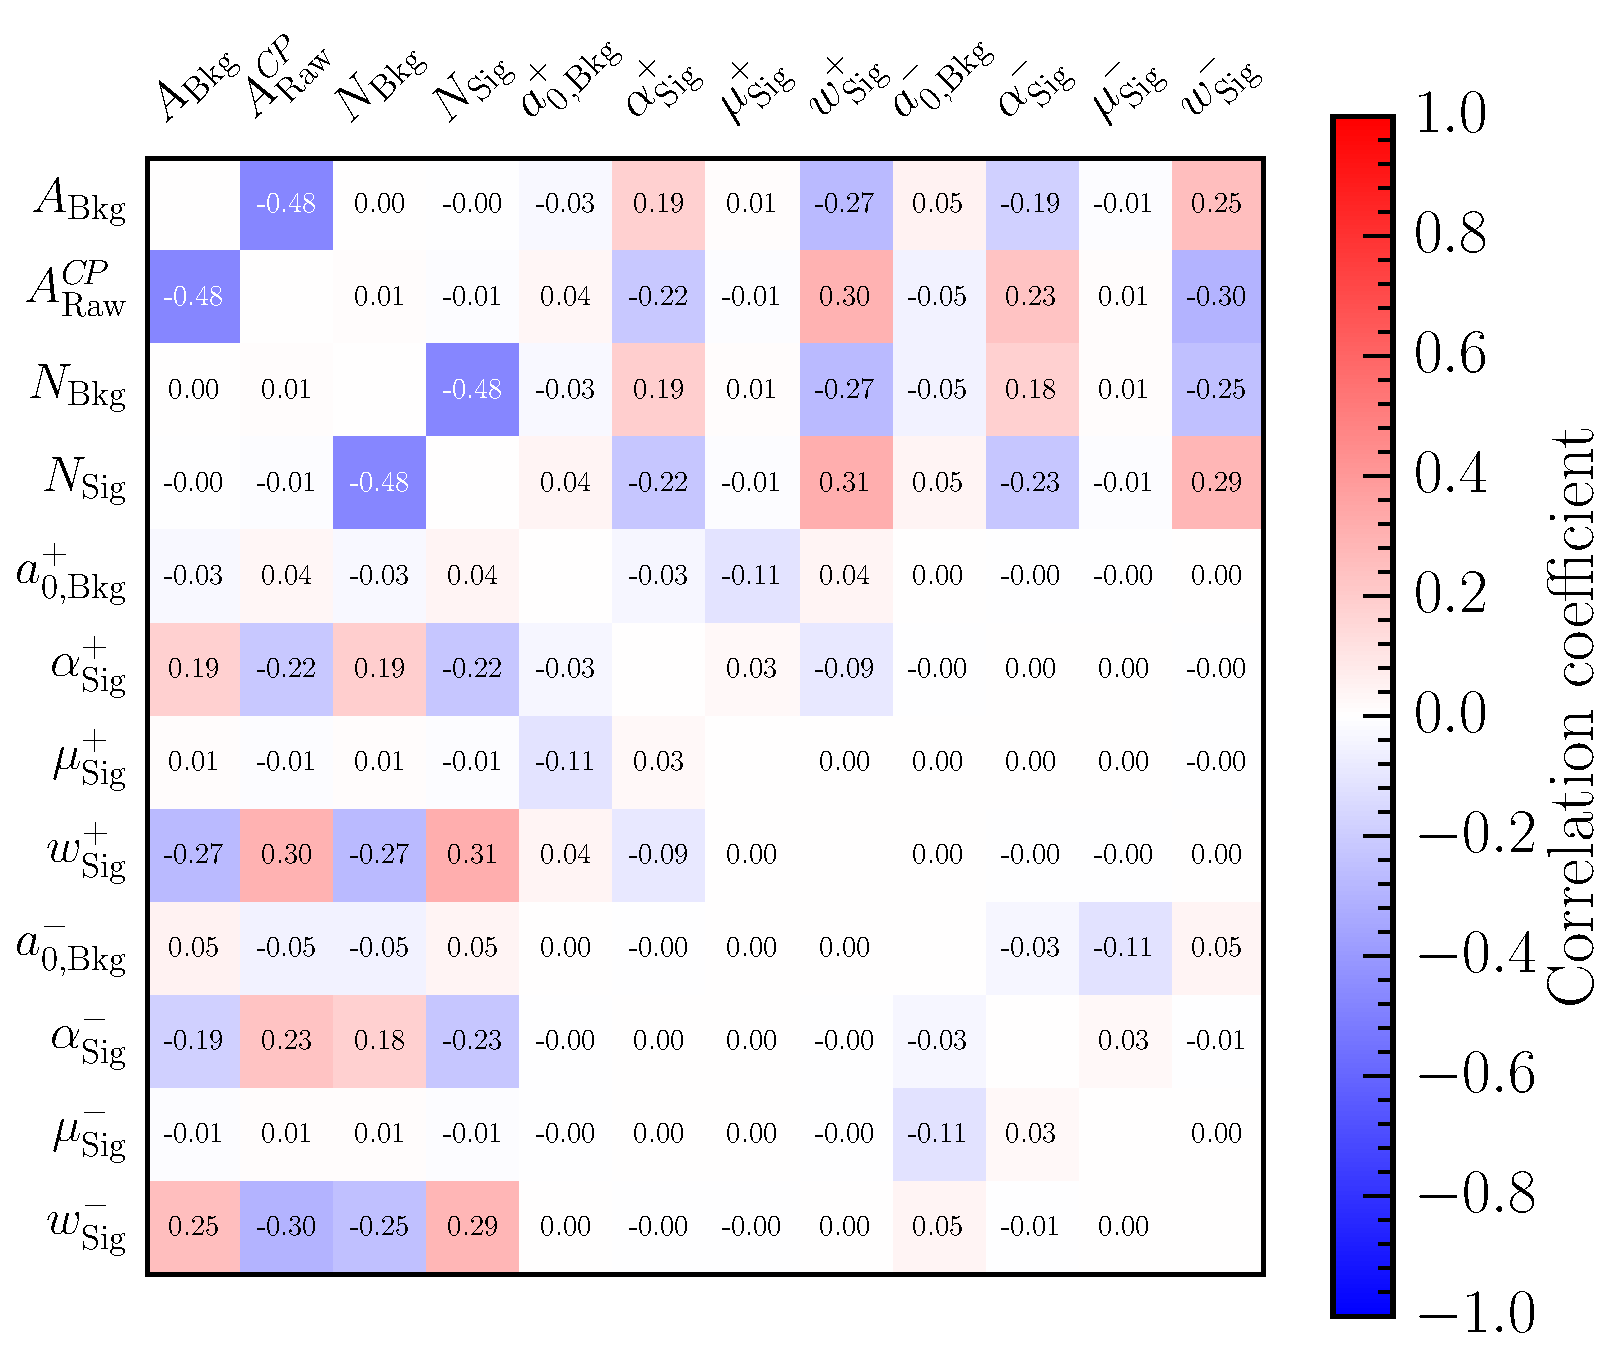
\includegraphics[width=\textwidth]{cpv/araw/LcToppipi_2012_MagDown_correlation_matrix.pdf}
      \caption{\ppipi}
      \label{fig:cpv:araw:correlation:ppipi}
    \end{subfigure}
  \end{center}
  \caption{%
    Correlation matrices for the fit parameters used in the simultaneous fit to 
    the \PLambdac\ and \APLambdac\ mass spectra in the fully selected 2012 
    magnet down dataset for \pKK~(\subref*{fig:cpv:araw:correlation:pKK}) and 
    \ppipi~(\subref*{fig:cpv:araw:correlation:ppipi}).
    The corresponding fits are shown in 
    \cref{fig:cpv:araw:fits:pKK,fig:cpv:araw:fits:ppipi}.
  }
  \label{fig:cpv:araw:correlation}
\end{figure}

\section{Validation}
\label{chap:cpv:araw:validation}

It has been shown in \cref{chap:cpv:prelim_fits:validation} that the 
measurements of the signal and background yields in the fits to the 
charge-combined data samples are not biased.
It remains to validate the simultaneous fit that has been described in this 
\namecref{chap:cpv:araw}.
This is done in using real data.
Using real data, the fits are performed with the charge of the \PLambdac\ 
candidate being randomly assigned.
The true values of \ARaw\ and \ARawBg\ should then be zero.
This checks for mistakes in the implementation of the fitter, and that the 
uncertainty on those parameters is not under- or overestimated.

\subsection{Null test}
\label{chap:cpv:araw:validation:null}

Fits as described in this \namecref{chap:cpv:araw} are performed on real data 
where the charge of the \PLambdac\ candidate is randomly assigned, with an 
equal probability of being assigned a positive or a negative charge.
One thousand permutations of the charge assignments are tested for each mode 
and data sub-sample, the fit is performed for each permutation and the value of 
\ARaw is recorded.
As with the studies described in \cref{chap:cpv:prelim_fits:validation}, the 
pull distributions of \ARaw\ should have a width of one, and the unblinded 
value should have a mean of zero.

% As the true value of \ARaw\ is known when a set of random chosen signs is used, 
% being zero, such a study could unblind the value of \ARaw, as an unbiased 
% fitter should measure \ARaw\ to be the value of the blinding offset.
% To prevent this, the blinding string for each mode is changed, such that the 
% blinding offset for this study is different to that used in the nominal fits.

The unblinded results of the charge permutation experiments are shown in 
\cref{fig:cpv:araw:validation:null:pKK,fig:cpv:araw:validation:null:ppipi} for 
the 2012 magnet down \pKK\ and \ppipi\ data.
The width of the pull distribution of \ARaw for both is consistent with unity, 
and the means are consistent with zero, indicating that the fit is unbiased.

\begin{figure}
  \begin{subfigure}[t]{0.32\textwidth}
    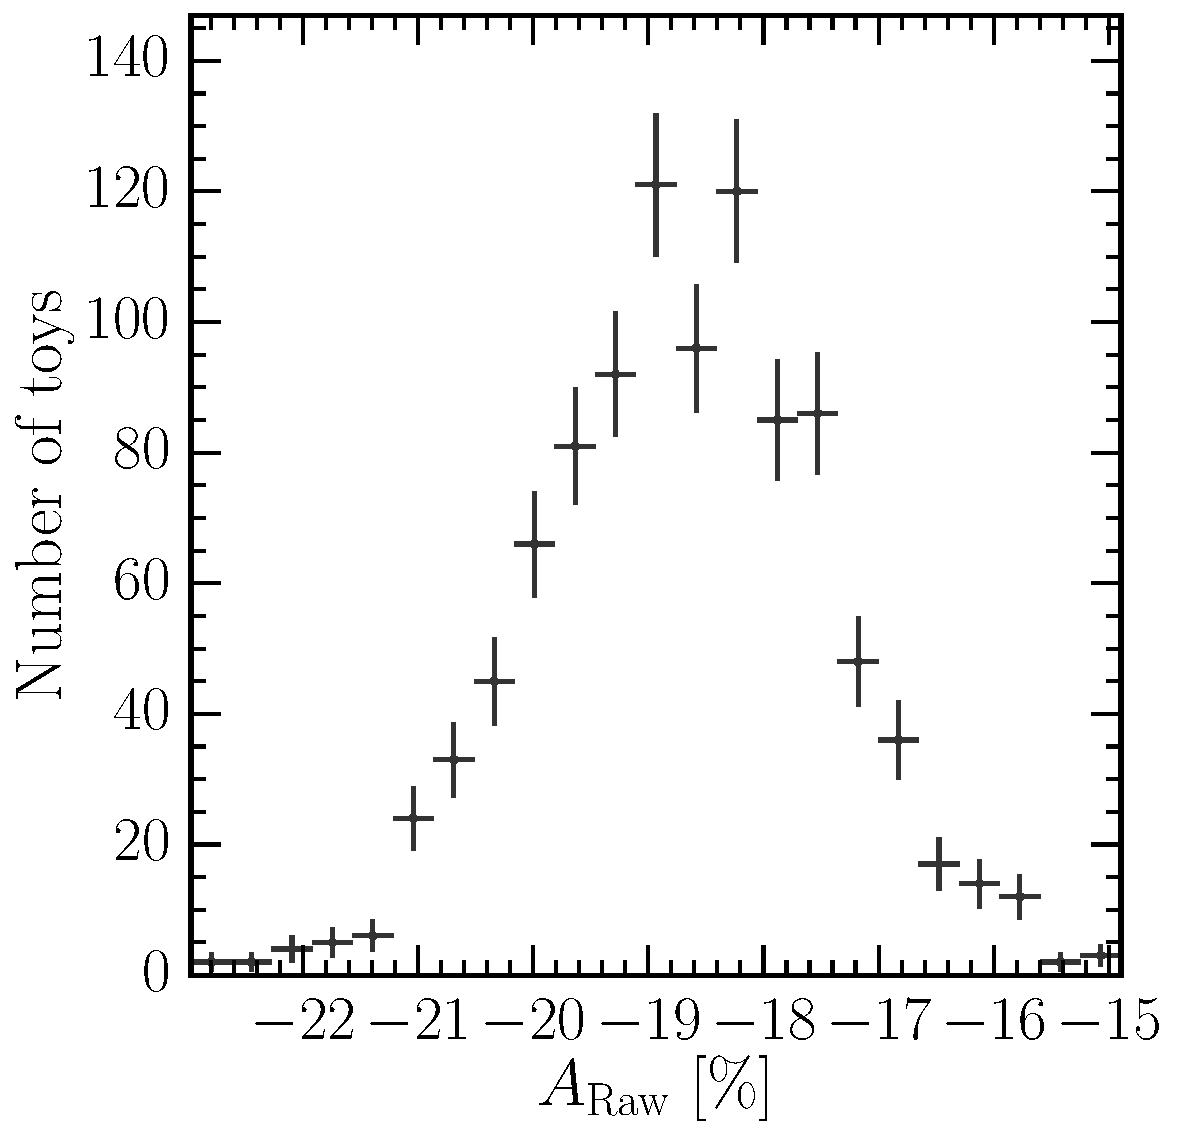
\includegraphics[width=\textwidth]{cpv/araw/validation/LcTopKK_2012_MagDown_araw.pdf}
    \caption{Values}
    \label{fig:cpv:araw:validation:null:pKK:values}
  \end{subfigure}
  \begin{subfigure}[t]{0.32\textwidth}
    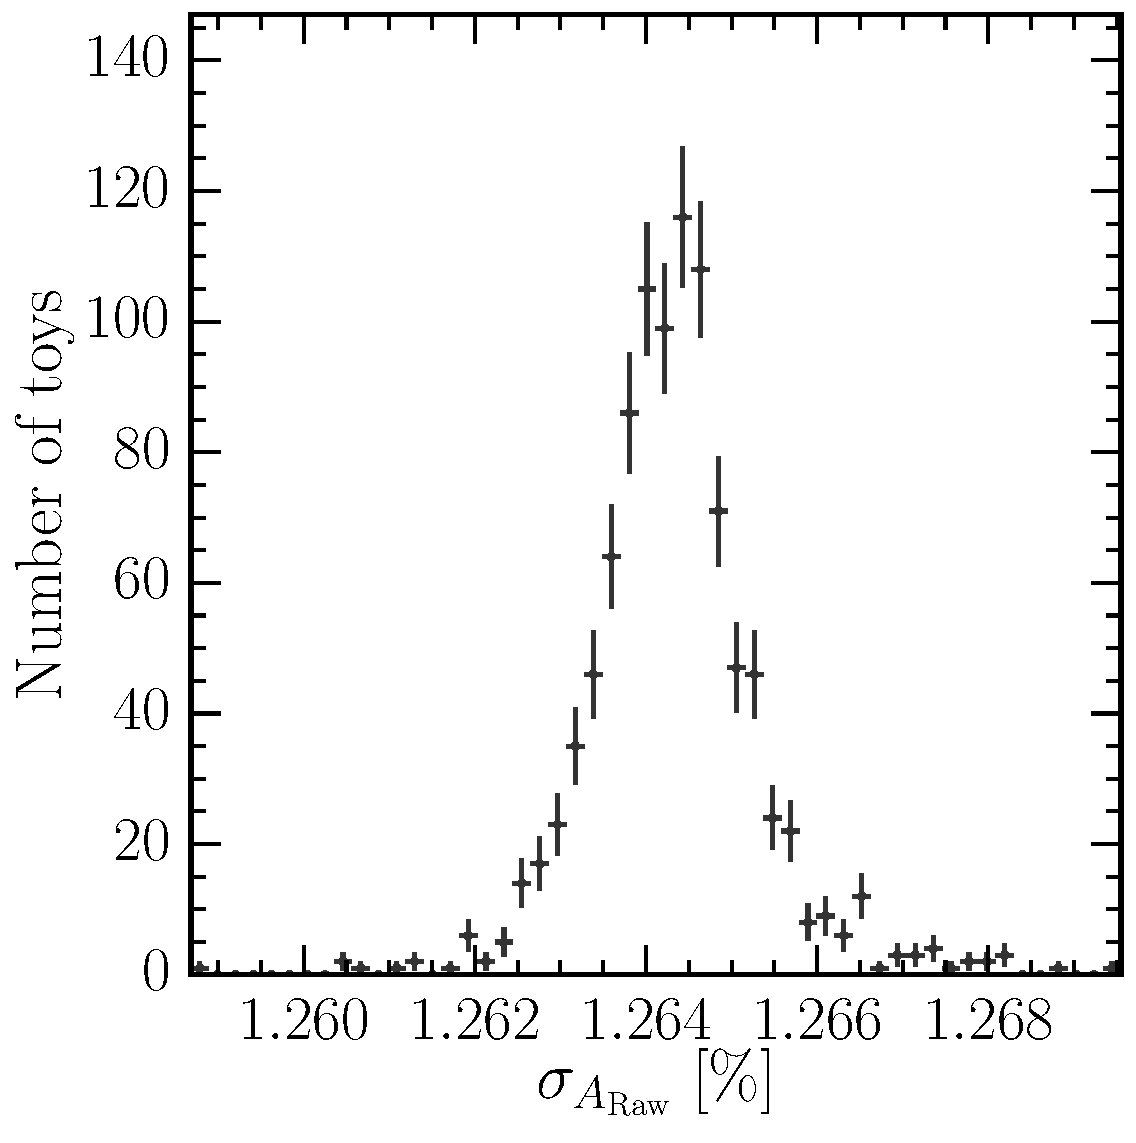
\includegraphics[width=\textwidth]{cpv/araw/validation/LcTopKK_2012_MagDown_araw_err.pdf}
    \caption{Errors}
    \label{fig:cpv:araw:validation:null:pKK:errors}
  \end{subfigure}
  \begin{subfigure}[t]{0.32\textwidth}
    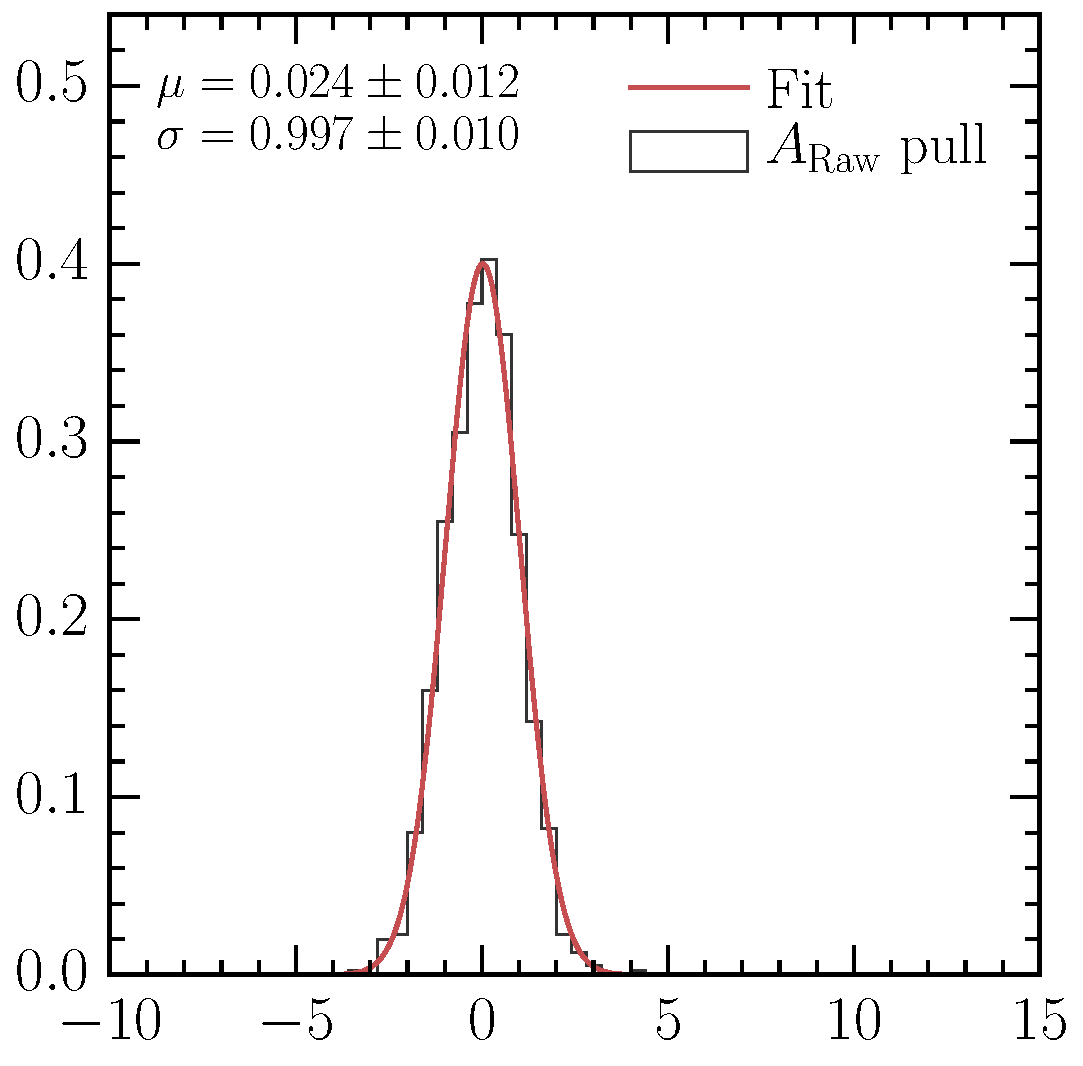
\includegraphics[width=\textwidth]{cpv/araw/validation/LcTopKK_2012_MagDown_araw_pull.pdf}
    \caption{Pulls}
    \label{fig:cpv:araw:validation:null:pKK:pulls}
  \end{subfigure}
  \caption{%
    Validation of the simultaneous fits to the \PLambdac\ and \APLambdac\ mass 
    spectra in the 2012 magnet down \pKK\ dataset, using randomly assigned 
    \PLambdac\ charges.
    The plots shows the distribution of the central values 
    (\subref*{fig:cpv:araw:validation:null:pKK:values}), uncertainties 
    (\subref*{fig:cpv:araw:validation:null:pKK:errors}), and pulls 
    (\subref*{fig:cpv:araw:validation:null:pKK:pulls}) of the \ARaw\ parameter, 
    assuming that the true value is zero.
    The pull distribution is overlaid with a fit of a Gaussian distribution 
    with mean $\mu$ and width $\sigma$.
  }
  \label{fig:cpv:araw:validation:null:pKK}
\end{figure}

\begin{figure}
  \begin{subfigure}[t]{0.32\textwidth}
    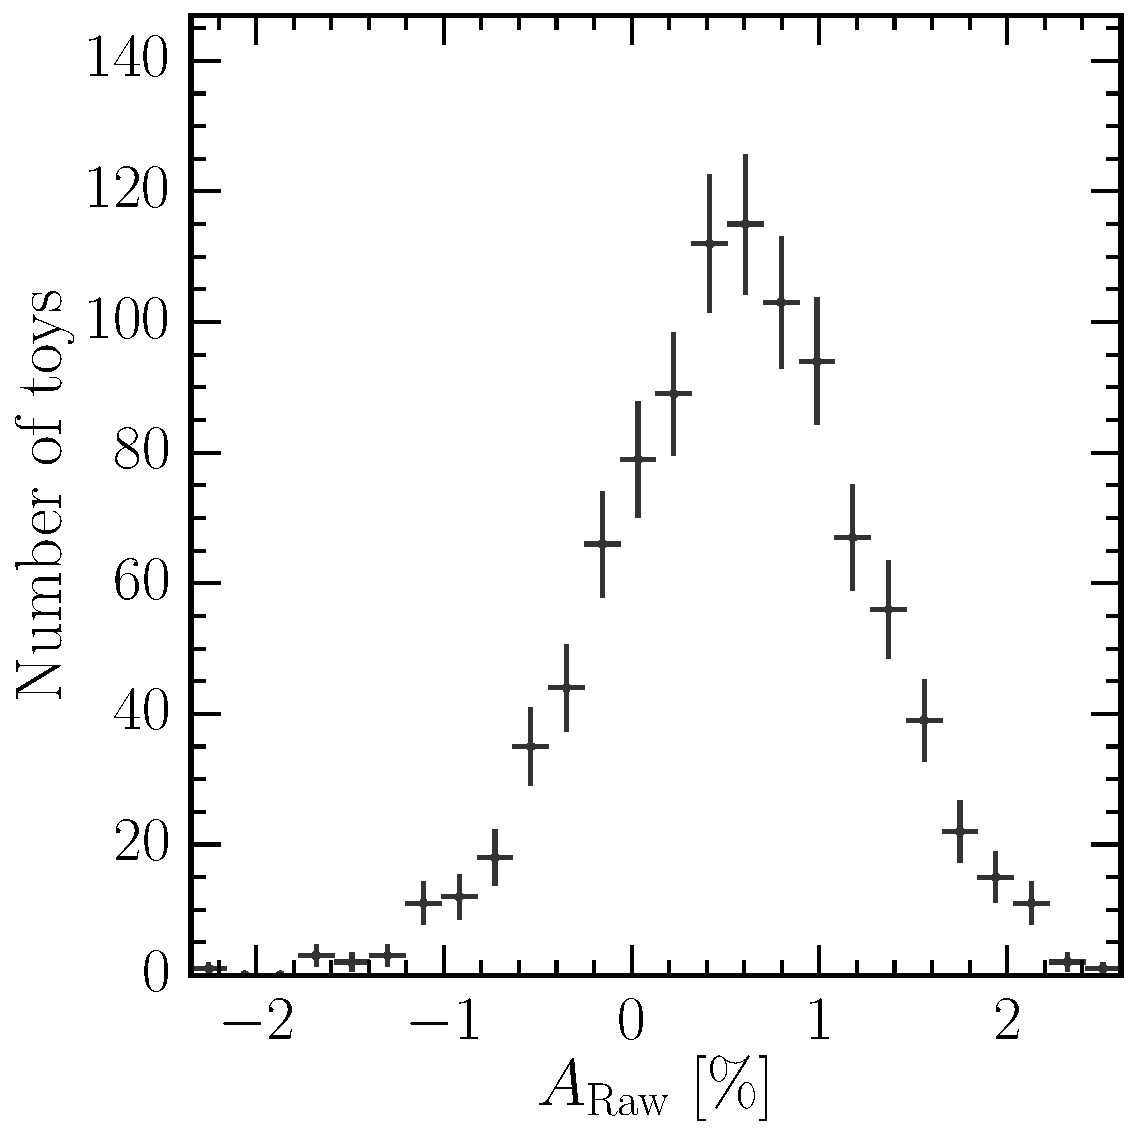
\includegraphics[width=\textwidth]{cpv/araw/validation/LcToppipi_2012_MagDown_araw.pdf}
    \caption{Values}
    \label{fig:cpv:araw:validation:null:ppipi:values}
  \end{subfigure}
  \begin{subfigure}[t]{0.32\textwidth}
    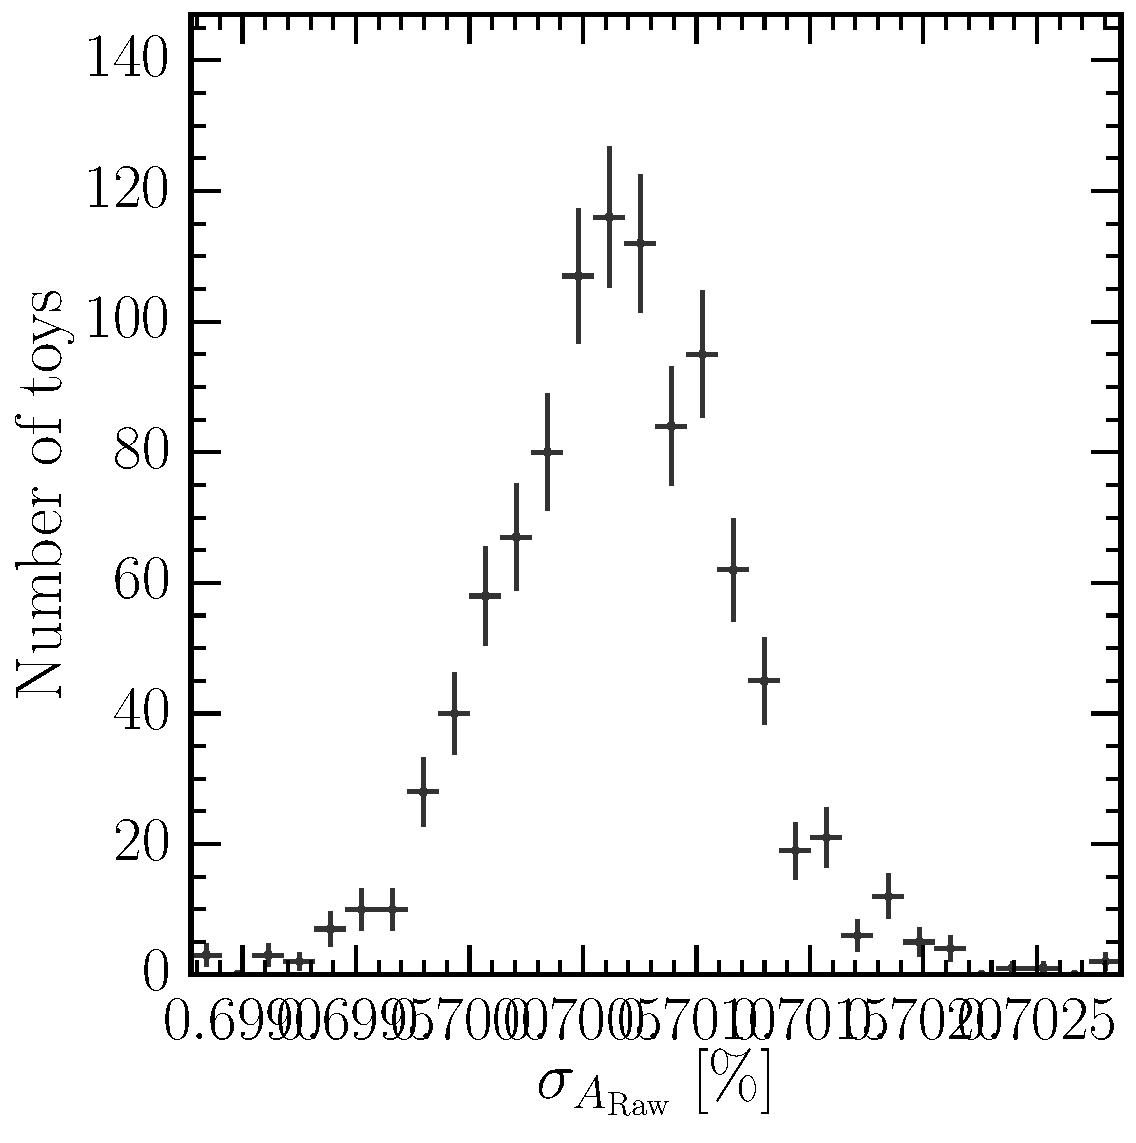
\includegraphics[width=\textwidth]{cpv/araw/validation/LcToppipi_2012_MagDown_araw_err.pdf}
    \caption{Errors}
    \label{fig:cpv:araw:validation:null:ppipi:errors}
  \end{subfigure}
  \begin{subfigure}[t]{0.32\textwidth}
    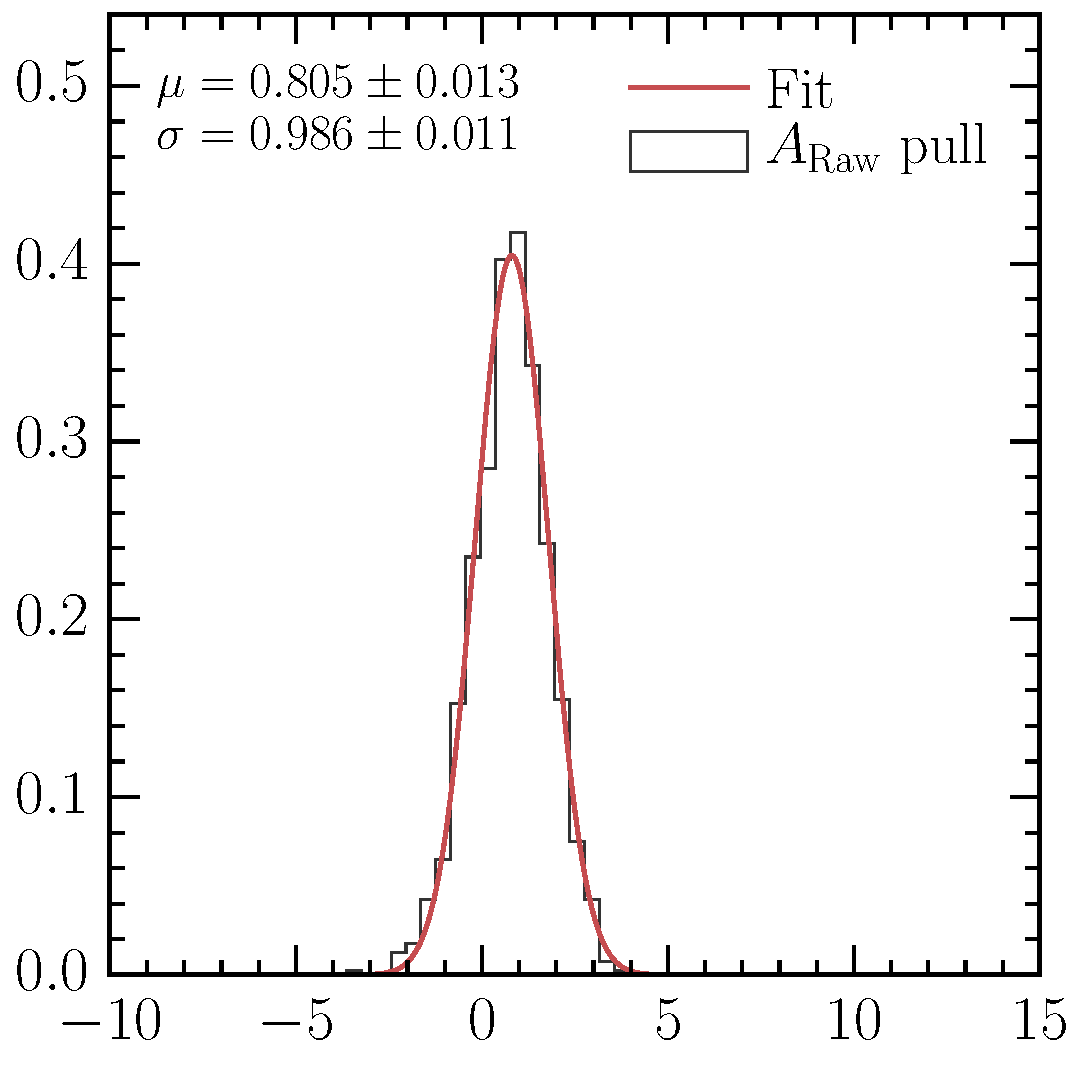
\includegraphics[width=\textwidth]{cpv/araw/validation/LcToppipi_2012_MagDown_araw_pull.pdf}
    \caption{Pulls}
    \label{fig:cpv:araw:validation:null:ppipi:pulls}
  \end{subfigure}
  \caption{%
    Validation of the simultaneous fits to the \PLambdac\ and \APLambdac\ mass 
    spectra in the 2012 magnet down \ppipi\ dataset, using randomly assigned 
    \PLambdac\ charges.
    The plots shows the distribution of the central values 
    (\subref*{fig:cpv:araw:validation:null:pKK:values}), uncertainties 
    (\subref*{fig:cpv:araw:validation:null:pKK:errors}), and pulls 
    (\subref*{fig:cpv:araw:validation:null:pKK:pulls}) of the \ARaw\ parameter, 
    assuming that the true value is zero.
    The pull distribution is overlaid with a fit of a Gaussian distribution 
    with mean $\mu$ and width $\sigma$.
  }
  \label{fig:cpv:araw:validation:null:ppipi}
\end{figure}
